The KNN algorithm was implemented by interpreting each feature, or in this case
every document, as a dimension and the feature values corresponds to the term
occurrence frequencies. Calculations of the nearest neighbours is
implemented in a non deterministic way. This because of that a point $x$ in a plane
may have neighbours with the property that they have equal distances to
$x$. If this is the case a nearest neighbour is chosen at random. Several choices
for $k$ was tested in different runs of the algorithm to find the best $k$ for
the classification. The algorithm was implemented to be able to classify both
different classes (music , software, etc.) and sentimental classification
(positive, negative). Figure \ref{fig:KNNplot} shows the misclassification done by the
algorithm for both different $k$ and different sizes for the feature sets.
\begin{figure}[h!]
\begin{center}
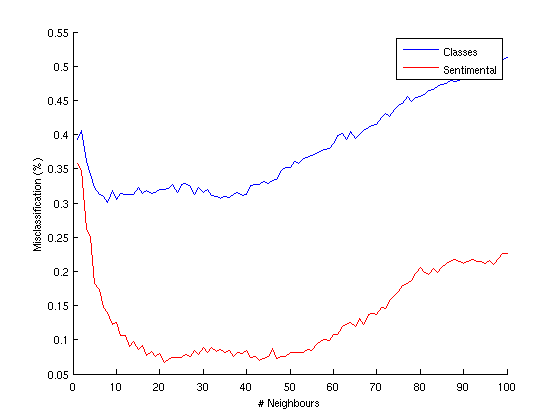
\includegraphics[scale=0.6]{fig/knn_2000words_testdata100_unigram}
\caption{Plot showing results from the KNN classifier}
\end{center}
\end{figure}
\label{fig:KNNplot}

Figure \ref{fig:KNNplot} shows that KNN has best performance with parameter  $K = 20$ for sentimental and $K = 10$ for classes.

%\begin{comment}
%The pseudocode below described the implemented matlab code.

%\begin{algorithm}[H]
% \SetKwData{Left}{left}\SetKwData{This}{this}\SetKwData{Up}{up}
% \SetKwFunction{Union}{Union}\SetKwFunction{FindCompress}{FindCompress}
% \SetKwInOut{Input}{input}\SetKwInOut{Output}{output}
% \Input{A data set X, A vector of labels Y,Number of nearest neigbour k,A feature vector x}
% \Output{A classification index}
% $\forall$ documents in data calculate the distances $D$ to $x$\;
% SDI = Sort the vector D and get the indexes in D \;
% S = A zero vector of size equal to the number of labels \;
%
% \For{i $\in$ \{1 \ldots k\}}{
%  read current\;
%  \eIf{understand}{
%   go to next section\;
%   current section becomes this one\;
%   }{
%   go back to the beginning of current section\;
%  }
% }
% \caption{How to write algorithms}
%\end{algorithm}
